\documentclass[10pt, a4paper]{article}
\usepackage[utf8]{inputenc}
\usepackage[UKenglish]{babel}
\usepackage{xcolor, graphicx}
\usepackage{makeidx}
\usepackage[scale=0.85]{sourcecodepro}
\usepackage{amsmath, amssymb, amsfonts}
\usepackage{microtype}
\usepackage{comment}
\usepackage{physics}
\usepackage{siunitx}
\usepackage{tikz}
\usepackage{minted}
\usepackage{bookmark}
\usepackage{geometry}
\usepackage[print=m, lang=python, verbose]{fortex}

\makeindex

\usetikzlibrary{decorations.markings}
\definecolor{fortexbg}{HTML}{F8F8F0}
\definecolor{fortextab}{HTML}{C0C0A8}
\usemintedstyle{ayu}
\setfortex{tabsize=2, breaksymbol=\scriptsize{$\hookrightarrow$}, fontsize=\small, breaklines, bgcolor=fortexbg, showtabs, tab={\rm{$\big|\hspace{0.825ex}$}}, tabcolor={fortextab}}
\DefineShortVerb{\"}

\begin{document}

\section{Introduction}

The aim of this code is to explore the idea of using a neural network for detecting magnetic monopoles in the LCHb rich1 detector. 

There are a few things that I have noted with a traditional NN that make it potentially problematic for this use case, and that is overconfidence. As it is unlikely that there will even be a monopole in the data, one of the important things is to make sure that we catch \emph{every} monopole. 

For this reason It was decided to use the fast NN as a cut for the slower, but more accurate Hough transform. 
However in order to do this we need the NN to not be overconfidence so we can take the $N$ most likely monopole candidates to then subsequentially run the hough transform over.

\section{Code}
\subsection{Initialisation}

\begin{code}
import logging
from ctypes import * 
import numpy as np
import imageio
import gc
import tensorflow as tf
import tensorflow_datasets as tfds
import tensorflow_probability as tfp
import matplotlib.pyplot as plt
from ROOT import TFile
\end{code}

First things first is we need to make sure that we can see a GPU. This is a non-trivial thing to do. 
On my OpenSuSe tumbleweed installation, I need 3 separate repos.
\begin{table}[h]
\begin{tabular}{|c|c|l|} \hline
 Description     & Intended Distro     & Url \\\hline
 Drivers \& Cuda & OpenSuSe tumbleweed & 
 \tiny\url{https://download.nvidia.com/opensuse/tumbleweed} \\\hline
 Advanced Cuda   & OpenSuSe leap       & 
 \tiny\url{https://developer.download.nvidia.com/compute/cuda/repos/opensuse15/x86_64} \\\hline
 cuDNN           & RHEL                & 
 \tiny\url{https://developer.download.nvidia.com/compute/cuda/repos/rhel8/x86_64/} \\\hline
\end{tabular}
\end{table}

Note that I also have the nvhpc repo (for sles) also installed for using cuda from fortran, but as far as I know that is not used here 

\begin{code}
print(tf.config.list_physical_devices('GPU'))
\end{code}

Finally we load our fake data generation library because doing it in python is just too darn slow. 
Note that we are wrapping the first argument in a list even though it will be length 1.

The prototype for "mk_griddata" is:

\begin{verbatim}
subroutine mk_griddata(N, d, l)
  integer(c_int),  intent(in)  :: N 
  integer(c_int),  intent(out) :: d(128, 128, N)
  logical(c_bool), intent(out) :: l(N)
end subroutine
\end{verbatim}

Note however that due to Fortran / C order the array dimensions for "d" need to be flipped. 

\begin{code}
so = CDLL("./nn_fake_gendata.so")
so.mk_griddata.argtypes = [np.ctypeslib.ndpointer(dtype=c_int,  ndim=1, flags="C"),
                           np.ctypeslib.ndpointer(dtype=c_int,  ndim=3, flags="C"),
                           np.ctypeslib.ndpointer(dtype=c_bool, ndim=1, flags="C")]
#so.loadroot.argtypes    = [c_char_p,
                           #c_size_t,
                           #np.ctypeslib.ndpointer(dtype=c_float, ndim=3, flags='C'),
                           #np.ctypeslib.ndpointer(dtype=c_double, ndim=1, flags='C'),
                           #np.ctypeslib.ndpointer(dtype=c_double, ndim=1, flags='C')]
so.loadroot.argtypes    = [c_size_t,
                           np.ctypeslib.ndpointer(dtype=c_float, ndim=3, flags='C')]
\end{code}

We are validating the monopole detections against some accurate simulation data that takes $\sim20$\si{\minute} for each monopole event to be generated, but is it more accurate than the faux data that I am generating using my random number generators. 

Note however that the data from the simulation is a bit funny as is my reconstruction of it. 

\begin{figure}[h]
\centering
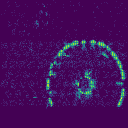
\includegraphics[width=0.3\textwidth]{Images/0.png}
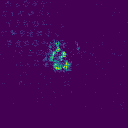
\includegraphics[width=0.3\textwidth]{Images/1.png}
\caption{Some examples of the simulated monopoles and the weird reconstruction}
\end{figure}

\begin{codeblock}{real_data}
\begin{code}
def real_data(n):
	print("getting real data from root file")
	d = np.zeros((n,128,128), dtype=c_float)
	#so.loadroot(c_char_p(bytes("../ns~Bender_monopole_10000.root", "utf8")), n, d, eta, beta)
	j = so.loadroot(n, d)
	print("Finished loading ", j, " elements")
	dd = d[:j-1, :, :]
	del(d)
	return dd 
\end{code}
\end{codeblock}

Here is where we generate the training data. note some interesting things here. We are basically doing manual memory management in python. This is because if we don't, we run out of memory real quick. (A dataset of $100,000$ images is about $6.5$ \si{\gibi \byte}). However As I have not found a way to load that memory into a dataset without performing a copy operation, you actually need $\sim14$\si{\gibi \byte} to work with it. 

Note also that the datasets need to be loading into tensorflow's special format for it to work correctly. 

Ideally I would like to make this a generator function instead of loading it all into memory (The other option is I just go and buy more RAM for my computer) However I don't know how to make tensorflow batch the calls to "mk_griddata" and still work with "yeild".

Finally another option is to save the training data to the disk as opposed to ram. This would slow down training however, It will allow for more training data to be used. However I need to figure out the format need for the data to work.

\begin{subfile}{python}{mk_dset.py}
\begin{code}
#! /usr/bin/env python3 

from ctypes import * 
import numpy as np
import tensorflow as tf
import sys

so = CDLL("./nn_fake_gendata.so")
so.mk_griddata.argtypes = [np.ctypeslib.ndpointer(dtype=c_int,  ndim=1, flags="C"),
                           np.ctypeslib.ndpointer(dtype=c_int,  ndim=3, flags="C"),
                           np.ctypeslib.ndpointer(dtype=c_bool, ndim=1, flags="C")]
i = int(sys.argv[1])

print(i)
train_n = np.ones(1, dtype=c_int) * 150000
train_d = np.zeros((train_n[0], 128, 128), dtype=c_int)
train_l = np.zeros(train_n[0], dtype=c_bool)

so.mk_griddata(train_n, train_d, train_l)
train_dset = tf.data.Dataset.from_tensor_slices((train_d, train_l))
tf.data.experimental.save(train_dset, "ns~tfr/"+str(i)+".tfr", compression='GZIP')
\end{code}
\end{subfile}

Note that if "compression" is not specified (or spelt wrong), or the "element_spec" has the wrong shape or type, then the model will fail to work. 
Specifically it will fail so silently that you will end up spending half an hour wondering why you are getting corruptions down the path. 
There is \emph{no} warning if the "element_spec" does not match. There is \emph{no} warning if gzip is lowercase instead up uppercase. 

\begin{codeblock}{mk_dset}
\begin{code}
def mk_dset():
	test_dset = tf.data.experimental.load("fastdata/ns~tfr/0.tfr",
	                                      element_spec = (tf.TensorSpec(shape=(128, 128), dtype=tf.int32),
	                                                      tf.TensorSpec(shape=(), dtype=tf.bool)),
	                                      compression='GZIP').batch(64).prefetch(1000)
	train_dset = tf.data.experimental.load("fastdata/ns~tfr/1.tfr",
	                                       element_spec = (tf.TensorSpec(shape=(128, 128), dtype=tf.int32),
	                                                       tf.TensorSpec(shape=(), dtype=tf.bool)),
	                                       compression='GZIP')
	for i in range(2,50):
		train_dset = train_dset.concatenate(tf.data.experimental.load("fastdata/ns~tfr/"+str(i)+".tfr",
	                                       element_spec = (tf.TensorSpec(shape=(128, 128), dtype=tf.int32),
	                                                       tf.TensorSpec(shape=(), dtype=tf.bool)),
	                                       compression='GZIP'))
	train_dset = train_dset.batch(64).prefetch(1000)
	return train_dset, test_dset
\end{code}

\begin{comment}
\begin{code}
	test_n = np.ones(1, dtype=c_int) * 1000
	test_d = np.zeros((test_n[0], 128, 128), dtype=c_int)
	test_l = np.zeros(test_n[0], dtype=c_bool)
	so.mk_griddata(test_n, test_d, test_l)
	test_dset = tf.data.Dataset.from_tensor_slices((test_d, test_l)).batch(64).prefetch(1000)
	
	del(test_n, test_d, test_l)
	gc.collect()
	
	train_n = np.ones(1, dtype=c_int) * 150000
	train_d = np.zeros((train_n[0], 128, 128), dtype=c_int)
	train_l = np.zeros(train_n[0], dtype=c_bool)
	so.mk_griddata(train_n, train_d, train_l)
	train_dset = tf.data.Dataset.from_tensor_slices((train_d, train_l)).batch(64).prefetch(1000)
	
	del(train_n, train_d, train_l)
	gc.collect()
	return train_dset, test_dset
\end{code}
\end{comment}
	
\end{codeblock}

\subsection{The Model}

Ugh I hate OOPify every mentality. 

\begin{codeblock}{callback}
\begin{code}
class callback(tf.keras.callbacks.Callback):
\end{code}

Here "on_epoch_end" is a magic function name that gets called at the end of each epoch. we will be using it to find the best epoch for validation. we can then plot this over the number of model parameters.

\begin{codeblock}{on_epoch_end}
\begin{code}
	def on_epoch_end(self, epoch, logs=None):
		fp = open("d.dat", 'a')
		print(logs.keys())
		if epoch == 0:
			fp.write("\n")
			self.model.summary(print_fn = lambda x: print(x, file=fp))
			fp.write("Validation loss, Validation Acc\n")
		fp.write(str(logs['val_loss']) + "\t" + str(logs['val_binary_accuracy']) + "\n")
		fp.close()
\end{code}
		
\end{codeblock}
\end{codeblock}

\begin{codevar}{checkpoint}
\begin{code}
checkpoint = tf.keras.callbacks.ModelCheckpoint(filepath="./fastdata/cp-{epoch:04d}.ckpt",
                                                 save_weights_only=True,
                                                 verbose=1)
\end{code}
\end{codevar}

Interestingly the first layer gets rid of the \oldstylenums{2}\textsc{d} image, and converts it to a \oldstylenums{1}\textsc{d} line. 
To me this is interesting as the algo now has to work out from scratch the original size of the image if it wants to find any vertical features. 

We then use some fully connected ``dense layers'', using a ``leaky rectified linear unit'' ("leaky_relu") activation function. 

\begin{equation}
f(x) = \begin{cases} x & x \geq 0 \\ \alpha x & x < 0 \end{cases}
\end{equation}

where $\alpha$ is a small number. I have found a leaky rectified linear unit to be batter than a regular one, and I am assuming that it is because there is always a non-zero gradient. 

one of the big problems with using relu's however is they are overconfident. and it has been proven that they will always be overconfident for data arbitrarily far away from the training data. This for us is problematic if we want to find all the monopoles, as it would be better if the model was uncertain about the data so we could shove that data though the Hough transform, before finally having a manual set of eyes look over the final 1000 or so images. 

To do create this uncertainty, two different techniques are used. The first is the use of dropout and regularisation. It has been shown that a model that uses these two techniques is actually an approximation of a beysian NN. In some iterations I did try going fully beysian however after spending a day trying to get it to work, I settled on this and it seems to be doing fine so whatever.

The second technique is using a Bernoulli distribution as the final layer. This is a probabilistic distribution that is defined:
\begin{equation}
 \text{\textsc{pdf}}_\text{B}(x; p) =  \begin{cases} (1-p) & x = 0 \\ p & x = 1 \end{cases}
\end{equation}

Some important properties about this distribution are: That all samples will be $X_i \in \{0, 1\}$, and for us we are interpreting $0$ as "False", and $1$ as "True". The mean $\mu$ of this distribution is $\mu = p$ and the standard deviation $\sigma$ is $\sigma = \sqrt{p(1-p)}$. 

As this is the final layer of the neural net, and the outcome of it is randomly sampled with the shape parameter $p$ is defined by the previous layer. 
Using this gives us an estimate of the uncertainty because it allows the neural net to minimise, but not forcibly go the the extremes.
\begin{codeblock}{main}
\begin{code}
def main():

	train_dset, test_dset = mk_dset()
	
	model = tf.keras.Sequential([
			tf.keras.layers.InputLayer(input_shape=(128,128)),
			tf.keras.layers.Flatten(),
			tf.keras.layers.Dense(20, activation='leaky_relu',
			                      kernel_regularizer=tf.keras.regularizers.l2(0.01)),
			tf.keras.layers.Dropout(0.2),
			tf.keras.layers.Dense(1, activation='leaky_relu'),
			tfp.layers.IndependentBernoulli(1, tfp.distributions.Bernoulli.logits)
	])
	model.summary()
\end{code}

We then `compile' the model. 

I have read in other sources that in general the "adam" optimiser is the best general optimiser, other optimisers can be better in specific situations, but this can be tweaked later. 

In this model because our final output is a distribution function and not a single number we can optimise log-likelihood. This allows us to avoid some of the problems with overconfidence as the ll function will auto correct if we overfit.


\begin{code}
	model.compile(
		optimizer=tf.keras.optimizers.Adam(1e-3),
		loss=lambda y, model: -model.log_prob(y),
		metrics=[
			tf.keras.metrics.BinaryAccuracy(threshold=0.5)
		],
	)
\end{code}

\subsection{Training}

One of the things that I have noticed from training is that in general that probabilistic approach tends to give $\sim99.7\%$ accuracy, but the classical approach gives $\sim99.95\%$. However, if we also take into account how many monopoles can be deduced from the uncertainty the accuracy drops as some non-monopoles get mixed into the data, but this is fine for as as we are going to run it though a Hough transform anyway and as long as we have all of the monopoles in the filtered dataset (i.e. no false negatives) we should be fine.

Note in the callbacks that one of them has brackets and one does not. Tensorflow requires callbacks that are classes to be a call and callbacks that are functions to not be. As for why checkpoint cannot be a regular function? who knows. 

\begin{code}
	print("Starting training")
	model.fit(train_dset, epochs=10, batch_size=64, callbacks=[checkpoint, callback()], validation_data=test_dset)
	model.save_weights("./fastdata/final.h5")
\end{code}
\begin{code}
	#print("loading model")
	#model.load_weights("./fastdata/64-10-nn.h5")
\end{code}
\begin{code}
	del(train_dset, test_dset)
	gc.collect()
\end{code}

\subsection{Accuracy and Plotting}

Here we are evaluating the performance of the model that we just trained. To do this to a degree of accuracy I am happy with I am clearing out the datasets and regenering them. 

We also save some of the newly generated data for plotting what is going on.

\begin{code}
	test_n = np.ones(1, dtype=c_int) * 3000
	test_d = np.zeros((test_n[0], 128, 128), dtype=c_int)
	test_l = np.zeros(test_n[0], dtype=c_bool)
	
	so.mk_griddata(test_n, test_d, test_l)
	
	pred_dist = model(test_d)
\end{code}

Let us now use these extra images to explicitly make predictions as opposed to just evaluation the performance. We do this so I can see the actual characteristics of the mode. i.e. is it confidently wrong, is it only confident when it is seeing monopoles, but middling otherwise, etc. 

We also do some plotting because why not.

\begin{code}
	pred_m = pred_dist.mean().numpy()
	pred_std = pred_dist.stddev().numpy()
	print(np.shape(pred_m), np.shape(pred_std))
	np.set_printoptions(formatter={'float_kind':"{:.4f}".format})
	print(pred_m)
\end{code}

Let us now look at the first 10 image we see.

\begin{code}
	minx = [np.min(pred_m - 1.96 * pred_std), np.max(pred_m + 1.96 * pred_std)]
	for i in range(10):
		#print(pred_mean[i], pred_std[i])
		plt.subplot(10,2,2*i+1)
		plt.imshow(test_d[i])
		plt.ylabel(str(test_l[i]), rotation='horizontal')
		plt.subplot(10,2,2*i+2)
		plt.plot(np.array([pred_m[i] + 1.96 * pred_std[i], pred_m[i] - 1.96 * pred_std[i]]), [0, 0], 'x')
		plt.plot(pred_m[i], 0, 'o')
		plt.ylim([-0.1,0.1])
		plt.xlim(minx)
		plt.gca().axes.get_yaxis().set_visible(False)
	plt.savefig("a.pdf", dpi=1600)
	
	p = (pred_m > 0.5)[:,0]
	for i in range(50):
		print(p[i], "\t", test_l[i], "\t", not (p[i] ^ test_l[i]), "\t", pred_m[i], pred_std[i])
	print("acc: ", np.sum(p == test_l), np.sum(p == test_l)/test_n)
	print("fp : ", np.sum(np.logical_and(p, np.logical_not(test_l))))
	print("fn : ", np.sum(np.logical_and(np.logical_not(p), test_l)))
	print("mst: ", np.mean(pred_std))
	plt.clf()
\end{code}

I really dislike how verbose matplotlib is and how hard it is to do anything however. all of this plotting nets us the image 

Let us also now look at some f the images that the NN explicitly got wrong. 

\begin{code}
	pred_std_s = np.flipud(np.unique(pred_std))
	test_d = test_d[np.logical_xor(p, test_l), :, :]
	pred_dist = pred_dist[np.logical_xor(p, test_l)]
	pred_m = pred_m[np.logical_xor(p, test_l)]
	pred_std = pred_std[np.logical_xor(p, test_l)]
	gc.collect()
	
	for i in range(len(test_d)):
		if i > 9:
			break
		plt.subplot(10,2,2*i+1)
		plt.imshow(test_d[i])
		plt.ylabel(str(pred_m[i])+"pm"+str(pred_std[i]), rotation='horizontal')
		plt.subplot(10,2,2*i+2)
		plt.plot(np.array([pred_m[i] + 1.96 * pred_std[i], pred_m[i] - 1.96 * pred_std[i]]), [0, 0], 'x')
		plt.plot(pred_m[i], 0, 'o')
		plt.ylim([-0.1,0.1])
		plt.xlim(minx)
		plt.gca().axes.get_yaxis().set_visible(False)
	plt.savefig("b.pdf", dpi=1600)
	
	for i in range(len(test_d)):
		print(pred_m[i] > 0.5, "\t", not (pred_m[i] > 0.5), "\t", pred_m[i], pred_std[i], np.argmax(pred_std_s == pred_std[i]))
		if i > 50:
			break
\end{code}

In general we see that all of these have very high uncertainty, and so will be easy to filter out and give to the Hough transform

Finally let us now test our code against data generated by loki and bender. This data is going to be much more similar to the data from the actual LHCb, but of course I don't actually have a lot of this data, so it is impractical to train the model on it.

\begin{code}
	plt.clf()
	img = real_data(36282)
	print(np.max(img))
	l = np.greater(np.sum(np.sum(img, axis=2), axis=1), 10)
	img_m = model(img).mean().numpy()
	img_s = model(img).stddev().numpy()
	print("Filter acc: 0.5: ", np.sum(np.equal((img_m[:,0] > 0.5), l)))
	print("Real acc: 0.5: ", np.sum(img_m > 0.5))
	print("Frac acc: 0.5: ", np.sum(img_m > 0.5)/len(img_m))
	print("      mean    stdv    guess   correct eta     beta")
	#     "Real: 0.11111 0.11111 [ True] [False] 0.11111 0.11111 
	for i in range(10):
		print("Real: %.5f %.5f %s %s" %
					(img_m[i], img_s[i], (img_m[i]>0.5), (img_m[i]>0.5) == l[i]) )
		plt.subplot(10,2,2*i+1)
		plt.imshow(img[i,:,:])
		plt.subplot(10,2,2*i+2)
		plt.plot(np.array([img_m[i] + 1.96 * img_s[i], img_m[i] - 1.96 * img_s[i]]), [0, 0], 'x')
		plt.plot(img_m[i], 0, 'o')
		plt.ylim([-0.1,0.1])
		plt.xlim(minx)
		plt.gca().axes.get_yaxis().set_visible(False)
	plt.savefig("d.pdf", dpi=1600)
	plt.clf()
	print("------------------------------------")
	s = np.flipud(np.argsort(img_m[:,0]))
	for i in range(10):
		print("Real: %.5f %.5f %s %s" %
					(img_m[s][i], img_s[s][i], (img_m[s][i]>0.5), (img_m[s][i]>0.5) == l[s][i]) )
		plt.subplot(10,2,2*i+1)
		plt.imshow(img[s,:,:][i,:,:])
		plt.subplot(10,2,2*i+2)
		plt.plot(np.array([img_m[s][i] + 1.96 * img_s[s][i], img_m[s][i] - 1.96 * img_s[s][i]]), [0, 0], 'x')
		plt.plot(img_m[s][i], 0, 'o')
		plt.ylim([-0.1,0.1])
		plt.xlim(minx)
		plt.gca().axes.get_yaxis().set_visible(False)
	plt.savefig("e.pdf", dpi=1600)
	plt.clf()
	
	#np.save("m.npy", img_m)
	#np.save("img.npy", img)
	#np.save("eta.npy", eta)
	#np.save("beta.npy", beta)
	#np.save("l.npy", l)
	
	#h1 = plt.hist2d( eta[l],
	                #beta[l],
	                #bins=50,
	                #range=[[np.min(eta), np.max(eta)],[np.min(beta), np.max(beta)]]
	                #)
	#h2 = plt.hist2d( eta[np.logical_and((img_m[:,0] > 0.5), l)], 
	                #beta[np.logical_and((img_m[:,0] > 0.5), l)],
	                #bins=50,
	                #range=[[np.min(eta), np.max(eta)],[np.min(beta), np.max(beta)]]
	                #)
	#plt.clf()
	#plt.imsave("etabeta1.png", (h2[0] + np.finfo(np.float64).eps)/(h1[0] + np.finfo(np.float64).eps))
	#plt.imsave("etabeta0.png", (h2[0])/(h1[0] + np.finfo(np.float64).eps))
	#plt.imsave("etabetae.png", np.sqrt(h1[0]))
	#print([[np.min(eta), np.max(eta)],[np.min(beta), np.max(beta)]])
	
\end{code}

And because python does not have an entry point function, we define out own. Side note: it has always annoyed me that python is so inflexible and does not support basic things like entry point functions and switch statements. Its like the worst of all worlds, inflexible like a static language, but the performance of a dynamic one.    

\begin{code}
if __name__ == "__main__":
	main()
\end{code}
\end{codeblock}

\printindex

\end{document}
 
